\documentclass[../projekt.tex]{subfiles}
\begin{document}

\chapter{Uživatelská příručka}

Tato aplikace slouží k~demonstraci Kargerova algoritmu. 

\section{Ovládání aplikace}


	\begin{figure}[ht]
    	\begin{center}
  			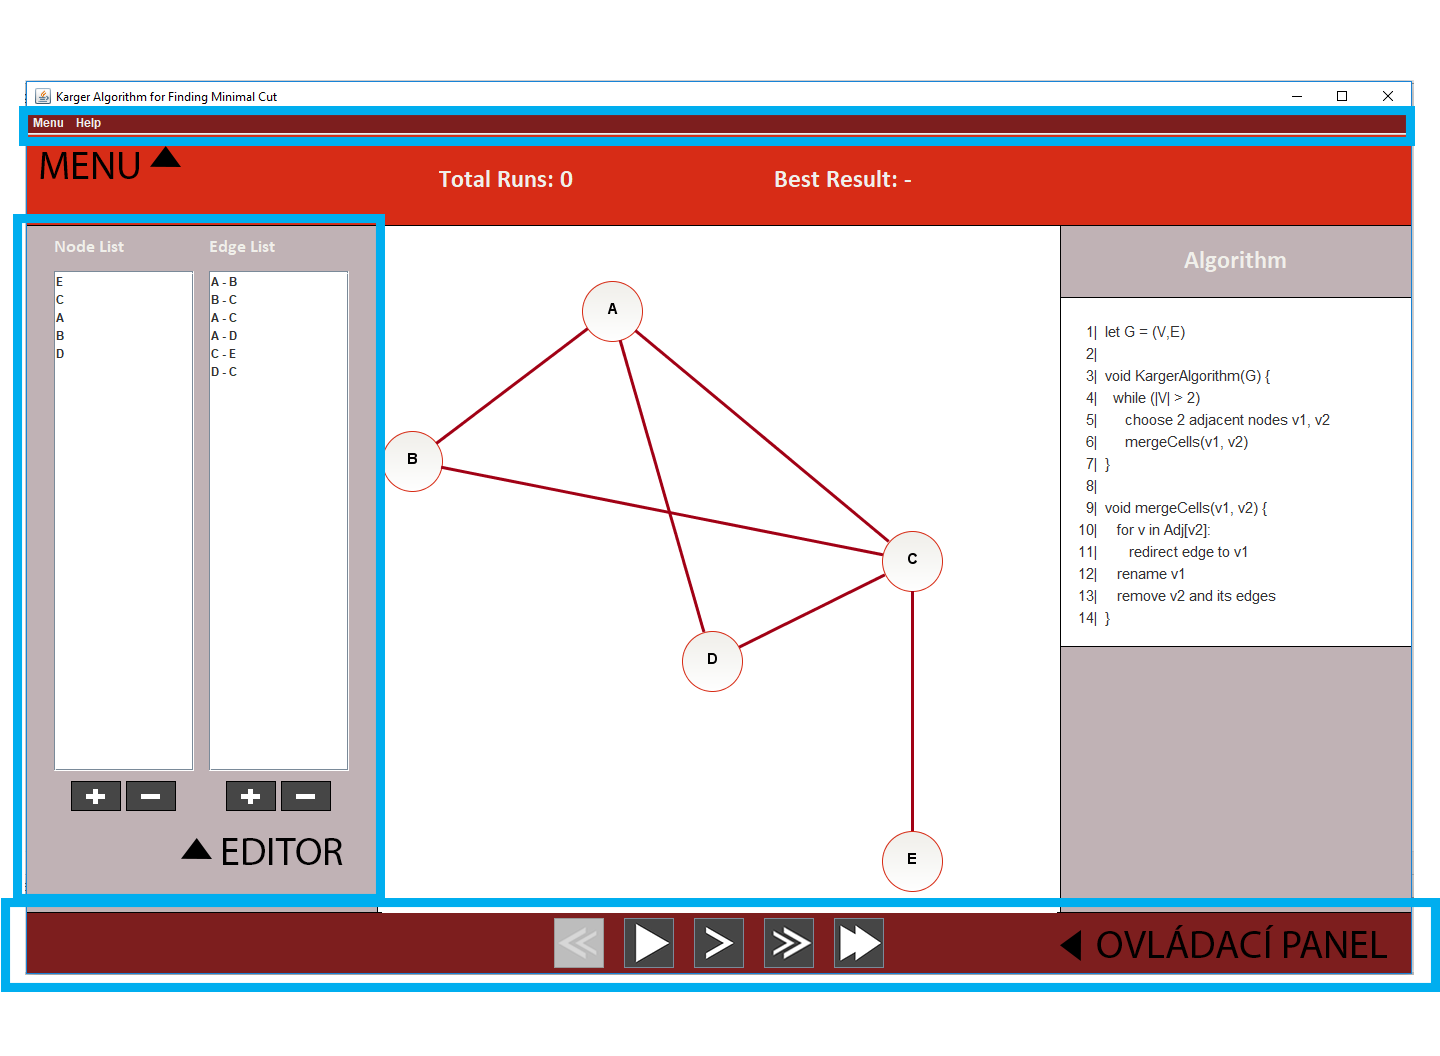
\includegraphics[scale=0.36]{obrazky-figures/ovladani.png}
  			\caption{Rozhraní ovládání aplikace.}
  		\end{center}
	\end{figure}
	
Aplikaci lze ovládat pomocí:
	
\begin{itemize}
	\item Menu -- Práce se souborem, nápověda.
	\item Editoru -- Úprava grafu.
	\item Ovládacího panelu -- Aplikace algoritmu na graf.
\end{itemize}


\subsection{Menu}

\begin{itemize}
    \item[] 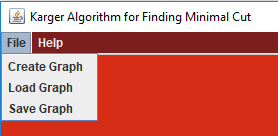
\includegraphics[height=10em]{obrazky-figures/file.png} \\Možnosti práce se souborem:
    \begin{itemize} \item vytvoření nového grafu
                    \item načtení uloženého grafu ve formátu XML
                    \item uložení grafu ve formátu XML
   \end{itemize}
    \item[] 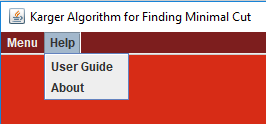
\includegraphics[height=10em]{obrazky-figures/help.png} \\Možnosti nápovědy:
    \begin{itemize} \item uživatelská příručka
                    \item o aplikaci
    \end{itemize}
\end{itemize}



\subsection{Editor}

Editor obsahuje seznam uzlů (\textit{Node List}) a seznam hran (\textit{Edge List}).
Ke každému z těchto seznamů jsou přidružena dvě tlačítka: 

\begin{itemize}
    \item[] 
\includegraphics[height=1.3em]{obrazky-figures/addButton.png} - Vložení uzlu/hrany do grafu
    \item[] 
\includegraphics[height=1.3em]{obrazky-figures/removeButton.png} - Odebrání uzlu/hrany z grafu \\
\end{itemize} 


\subsection{Ovládací panel}

Ovládací panel obsahuje pět různých tlačítek, přičemž aplikace může běžet
ve dvou různých módech. První tlačítko zleva je:  

\begin{itemize}
    \item[] 
\includegraphics[height=1.3em]{obrazky-figures/resetSmall.png} -- Resetování grafu.
    Vrátí graf do počátečního stavu a umožňuje začít znovu. 
\end{itemize}

\newpage

\noindent Zbývající čtyří tlačítka pracují v různých módech aplikace:

\subsubsection {Tzv. Single Run Mode}

\begin{itemize}
    \item[] 
\includegraphics[height=1.3em]{obrazky-figures/playSmall.png} -- Kliknutím na toto tlačítko dojde k provedení jednoho kroku algoritmu, tedy ke sloučení jedné dvojice uzlů a zobrazení aktualizovaného grafu.
    \item[] 
\includegraphics[height=1.3em]{obrazky-figures/nextStepSmall.png} -- Kliknutím na toto tlačítko dojde ke spuštění jednoho běhu algoritmu a zobrazení výsledku tohoto běhu.
    \item[] 
\includegraphics[height=1.3em]{obrazky-figures/manualSteps.png} -- Kliknutím na toto tlačítko je aktivováno manuální krokování algoritmu v pravém panelu, doprovázeno zobrazováním změn na grafu.
\end{itemize}

\subsubsection{Multiple Runs Mode}

\begin{itemize}
	\item[] 
\includegraphics[height=1.3em]{obrazky-figures/finishSmall.png} -- Kliknutím na dané tlačítko je spuštěn kompletní běh algoritmu.
\end{itemize}
Algoritmus tedy proběhne pro všechny možné varianty. Po dokončení zobrazí graf v počátečním stavu, nejlepší možný výsledek a všechny další výsledky.
\end{document}

